\documentclass[12pt]{article}

\usepackage{sbc-template}
\usepackage{graphicx,url}
\usepackage[utf8]{inputenc}
\usepackage[english]{babel}
\usepackage{amsmath}
\usepackage{amssymb}
\usepackage{booktabs}
\usepackage{multirow}
\usepackage{array}
\usepackage{xcolor}
\usepackage{colortbl}
\usepackage{tikz}
\usetikzlibrary{shapes.geometric, arrows.meta, positioning, fit, backgrounds}
\usepackage{enumitem}
\setlist{itemsep=0.5em}
\usepackage{indentfirst}
\usepackage{float}

\sloppy
\raggedbottom

\title{The Effect of Meta-Target Scaling on the Performance of Meta-Learning Systems for Algorithm Selection}

\author{Lael de Lima Santa Rosa\inst{1}}

\address{Computing Institute -- Federal University of Alagoas (UFAL)\\
  Macei\'o -- AL -- Brazil
  \email{llsr@ic.ufal.br}
}

\begin{document}

\maketitle

\begin{abstract}
Algorithm selection in machine learning frequently relies on meta-learning, where a meta-model learns to predict the performance of base algorithms from dataset characteristics (meta-features). However, the performance scores constituting the meta-target vary substantially in scale and distribution, raising the fundamental question of whether target preprocessing and scaling techniques affect meta-model performance. Inspired by Amorim et al. (2022), who demonstrated that the choice of scaling technique matters for base-level classification, this work investigates whether this principle holds at the meta-level. We evaluate four meta-models (Ridge, SVR, Random Forest, MLP) combined with five meta-target transformation and preprocessing strategies (Baseline, StandardScaler, MinMaxScaler, RobustScaler, QuantileTransformer) across four experimental scenarios: 50 controlled datasets, 144 and 200 real-world OpenML datasets characterized by 8 statistical meta-features, and the same datasets expanded to 78 descriptors via PyMFE. The results demonstrate that target scaling sensitivity is fundamentally governed by meta-model architecture: MLP collapses without target standardization (StandardScaler or RobustScaler), yielding a Spearman correlation of merely 0.03 on real-world data and a base-level performance below random choice; SVR substantially improves recommendation quality under robust standardization (RobustScaler), outperforming the best static heuristic; Random Forest remains invariant to linear scalers; and QuantileTransformer degrades ranking capability across most meta-models. Base-level evaluation proves that meta-target transformation governs the practical utility delivered to the end-user, while richer meta-features drastically reduce prediction errors across all models. No single scaling technique universally dominates.
\end{abstract}

% ============================================================
\section{Introduction}
% ============================================================

Machine learning (ML) algorithm selection is one of the most resource-intensive stages in building intelligent systems. Rather than exhaustively evaluating every candidate algorithm on a new dataset---an approach that is computationally prohibitive in terms of time and resources---\textit{meta-learning} leverages historical empirical performance to train a meta-model that maps dataset characteristics (\textit{meta-features}) to base algorithm performances (\textit{meta-target}), enabling the recommendation of the most suitable algorithm for unseen tasks~\cite{vanschoren2018meta}.

While input \textit{meta-features} typically undergo rigorous preprocessing and scaling, the performance scores forming the \textit{meta-target} are overwhelmingly utilized in their raw, untransformed form. Nonetheless, performance metrics such as macro-F1 exhibit substantial variation in both scale and distribution across diverse tasks, and this dispersion can severely hinder meta-models sensitive to scale discrepancies. The study by \cite{amorim2022choice} demonstrated at the base level that \textit{``the choice of scaling technique matters for classification performance''}---this work transposes the very same inquiry to the meta-level.

\textbf{Problem Formulation:} Does the scaling and transformation of the meta-target in meta-learning systems for algorithm selection yield meaningful performance differences? Is there a universal scaling recommendation suitable for any meta-model architecture?

\textbf{Hypotheses:} (H1) Meta-models sensitive to target scaling will display statistically significant performance variations across techniques. (H2) Tree-based meta-models will remain invariant to linear target transformations. (H3) No single target preprocessing technique will universally dominate across all meta-models.

\textbf{Main Contributions:}
\begin{itemize}
  \item The first systematic investigation into the impact of \textit{meta-target} scaling and transformation (as opposed to meta-feature scaling) in meta-learning systems;
  \item Demonstration that MLP severely collapses without meta-target standardization of $Y$, yielding recommendations no better than random guessing on real-world datasets even when input meta-features $X$ are standardized---a failure mode resolved by eliminating the target mean bias via StandardScaler or RobustScaler;
  \item Novel base-level evaluation demonstrating that SVR with RobustScaler outperforms the best static baseline (Single Best) and curtails average regret against the Ideal Oracle to $0.018$, whereas unscaled MLP collapses below random selection;
  \item Identification of QuantileTransformer as detrimental to ranking ability across the majority of meta-models;
  \item Validation across four progressive scenarios: controlled synthetic benchmarks, 144 and 200 real-world OpenML datasets characterized by 8 statistical meta-features, and the same 200 datasets expanded to 78 descriptors via the PyMFE library;
  \item Empirical demonstration that comprehensive meta-feature sets substantially reduce prediction error across all evaluated meta-models.
\end{itemize}

% ============================================================
\section{Proposed Approach}
% ============================================================

\subsection{Problem Formulation}

Let $\mathcal{D} = \{d_1, \dots, d_N\}$ denote a benchmark repository of $N$ classification datasets. For each dataset $d_i$, we extract a $D$-dimensional meta-feature vector $\mathbf{x}_i \in \mathbb{R}^D$, forming the meta-feature matrix $X \in \mathbb{R}^{N \times D}$. We evaluate a portfolio of $M$ base classification algorithms $\mathcal{A} = \{a_1, \dots, a_M\}$ on each dataset, yielding a performance vector $\mathbf{y}_i \in \mathbb{R}^M$ (e.g., the macro-F1 score of each algorithm $a_j$ on $d_i$) and the resulting meta-target matrix $Y \in \mathbb{R}^{N \times M}$. The objective is to induce a mapping $f$ that predicts $\hat{\mathbf{y}}_i \approx \mathbf{y}_i$ given $\mathbf{x}_i$, subsequently recommending the base algorithm with the highest estimated performance for an unseen dataset.

\subsection{Meta-Learning Pipeline with Meta-Target Transformation}

The core contribution of this work lies in examining the effect of a transformation $S: \mathbb{R}^{N \times M} \rightarrow \mathbb{R}^{N \times M}$ applied column-wise to $Y$ \textit{prior} to meta-model training. Figure~\ref{fig:pipeline} illustrates the proposed pipeline.

\begin{figure}[ht]
\centering
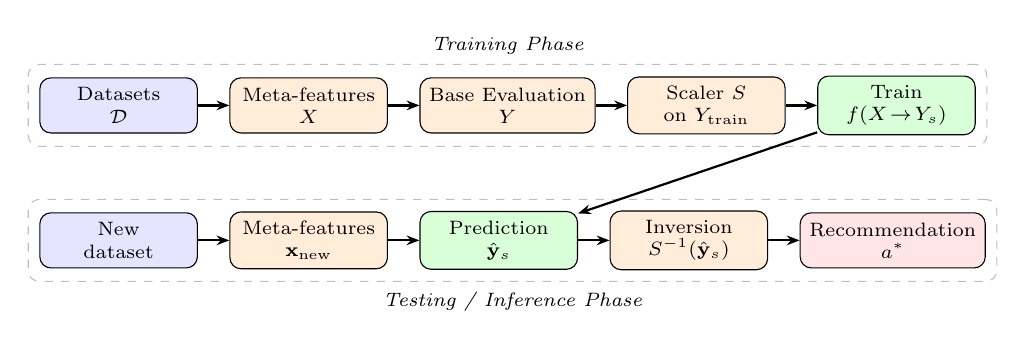
\begin{tikzpicture}[
  node distance=0.5cm and 0.4cm,
  box/.style={draw, rounded corners, minimum width=2.0cm, minimum height=0.7cm,
              font=\scriptsize, align=center, fill=white},
  databox/.style={box, fill=blue!10},
  procbox/.style={box, fill=orange!15},
  modelbox/.style={box, fill=green!15},
  evalbox/.style={box, fill=red!10},
  arr/.style={-{Stealth[scale=0.7]}, thick},
  phase/.style={draw=gray!50, dashed, rounded corners, inner sep=4pt}
]

% Nodes – Train phase
\node[databox]  (datasets)  {Datasets\\ $\mathcal{D}$};
\node[procbox,  right=of datasets]  (mf)    {Meta-features\\ $X$};
\node[procbox,  right=of mf]        (perf)  {Base Evaluation\\ $Y$};
\node[procbox,  right=of perf]      (scale) {Scaler $S$\\ on $Y_{\text{train}}$};
\node[modelbox, right=of scale]     (train) {Train\\ $f(X \!\to\! Y_s)$};

% Nodes – Test phase (below)
\node[databox,  below=1.0cm of datasets] (newds)  {New\\ dataset};
\node[procbox,  right=of newds]          (newmf)  {Meta-features\\ $\mathbf{x}_{\text{new}}$};
\node[modelbox, right=of newmf]          (pred)   {Prediction\\ $\hat{\mathbf{y}}_s$};
\node[procbox,  right=of pred]           (inv)    {Inversion\\ $S^{-1}(\hat{\mathbf{y}}_s)$};
\node[evalbox,  right=of inv]            (rec)    {Recommendation\\ $a^*$};

% Arrows – Train
\draw[arr] (datasets) -- (mf);
\draw[arr] (mf)       -- (perf);
\draw[arr] (perf)     -- (scale);
\draw[arr] (scale)    -- (train);

% Arrows – Test
\draw[arr] (newds)  -- (newmf);
\draw[arr] (newmf)  -- (pred);
\draw[arr] (train)  -- (pred);
\draw[arr] (pred)   -- (inv);
\draw[arr] (inv)    -- (rec);

% Phase boxes
\begin{scope}[on background layer]
  \node[phase, fit=(datasets)(mf)(perf)(scale)(train),
        label={[font=\scriptsize\itshape]above:Training Phase}] {};
  \node[phase, fit=(newds)(newmf)(pred)(inv)(rec),
        label={[font=\scriptsize\itshape]below:Testing / Inference Phase}] {};
\end{scope}
\end{tikzpicture}
\caption{Meta-learning pipeline incorporating meta-target transformation. The preprocessor $S$ is fitted strictly on the training partition, preventing data leakage. Post-prediction inversion $S^{-1}$ ensures that evaluation metrics remain on the original macro-F1 scale.}
\label{fig:pipeline}
\end{figure}

\subsection{Meta-Target Transformation and Scaling Techniques}

Five target preprocessing strategies applied column-wise to the meta-target matrix $Y$ represent distinct data transformation paradigms:
\begin{enumerate}
  \item \textbf{Baseline} (Raw data): $\tilde{y} = y$. Untransformed control group retaining the original performance values (macro-F1);
  \item \textbf{StandardScaler} (\textbf{Z-score Standardization}): $\tilde{y} = (y - \mu) / \sigma$. Centers data around zero mean ($\mu=0$) with unit variance ($\sigma=1$), aiding gradient descent stability;
  \item \textbf{MinMaxScaler} (\textbf{Min-Max Normalization}): $\tilde{y} = (y - y_{\min}) / (y_{\max} - y_{\min})$. Linearly bounds values to the closed interval $[0, 1]$, preserving the original distributional shape and relative distances, but retaining a positive offset mean;
  \item \textbf{RobustScaler} (\textbf{Robust Standardization}): $\tilde{y} = (y - \text{median}) / \text{IQR}$. Employs outlier-robust statistics (zero median and scaling via the interquartile range $Q_3 - Q_1$), preventing extreme performance values from skewing the distribution;
  \item \textbf{QuantileTransformer} (\textbf{Quantile Transformation}): $\tilde{y} = \Phi^{-1}\!\left( \frac{\text{rank}(y)}{n+1} \right)$. Maps data non-linearly to a standard normal distribution via the empirical quantile function, mitigating extreme skewness but distorting relative inter-rank distances.
\end{enumerate}

A fundamental mathematical distinction separates these families: StandardScaler and RobustScaler perform \textbf{standardization} (centering with zero mean or median followed by dispersion scaling), a property crucial for stabilizing gradient backpropagation and preventing neuron saturation in neural networks. In contrast, MinMaxScaler is strictly a \textbf{range normalization} that compresses scores into $[0, 1]$ without removing the non-zero bias offset (the mean remains around $0.65$ in our benchmark). Techniques 1--4 are strictly \textbf{monotonic} (preserving relative order), whereas quantile transformation is \textbf{non-linear} and may alter the ranking hierarchy among algorithms.

\subsection{Evaluation Metrics}

Pipeline evaluation is conducted across two complementary dimensions: the \textbf{meta-level} (meta-model predictive precision and ranking fidelity) and the \textbf{base-level} (practical utility and empirical performance delivered to the end-user).

\subsubsection{Meta-Level Metrics}
\begin{itemize}
  \item \textbf{MAE}: Mean Absolute Error evaluated on the original macro-F1 scale;
  \item \textbf{Spearman} ($\rho_s$): Rank correlation between predicted and true rankings of the $M$ base algorithms (ranging in $[-1, +1]$);
  \item \textbf{Acc@1}: Top-1 accuracy, representing the fraction of datasets where the top-predicted algorithm matches the true empirical winner.
\end{itemize}

\subsubsection{Base-Level Metrics}
To measure the concrete utility perceived by a practitioner, let $\mathbf{y}_i \in \mathbb{R}^M$ denote the true macro-F1 vector across the $M$ base algorithms on test dataset $i$, and let $j^*(i) = \arg\max_{j \in \{1, \dots, M\}} \hat{y}_{i, j}$ be the index of the base algorithm recommended at the top of the ranking by the meta-model. We evaluate:
\begin{itemize}
  \item \textbf{Average Base-Level F1 ($\overline{P}_{\text{base}}$):} The expected performance achieved by following the meta-model's recommendation:
  \begin{equation}
    \overline{P}_{\text{base}} = \frac{1}{N} \sum_{i=1}^N y_{i, j^*(i)}
  \end{equation}
  \item \textbf{Ideal Oracle ($\overline{P}_{\text{oracle}}$):} The theoretical performance upper bound obtained by perfectly selecting the optimal classifier for each dataset:
  \begin{equation}
    \overline{P}_{\text{oracle}} = \frac{1}{N} \sum_{i=1}^N \max_{j} y_{i, j}
  \end{equation}
  \item \textbf{Average Regret ($\overline{\text{Regret}}$):} The expected performance penalty incurred due to suboptimal recommendations:
  \begin{equation}
    \overline{\text{Regret}} = \overline{P}_{\text{oracle}} - \overline{P}_{\text{base}} = \frac{1}{N} \sum_{i=1}^N \left( \max_{j} y_{i, j} - y_{i, j^*(i)} \right)
  \end{equation}
  \item \textbf{Gain over Static Baselines:} We benchmark $\overline{P}_{\text{base}}$ against two static reference strategies requiring no meta-learning: \textit{Single Best} (consistently choosing the classifier with the highest historical training mean, Random Forest) and \textit{Random Choice}.
\end{itemize}

% ============================================================
\section{Experimental Methodology}
% ============================================================

\subsection{Datasets}

Four distinct experimental setups were conducted:

\textbf{Experiment 1 (controlled):} 50 classification datasets --- 4 real-world benchmarks from \texttt{scikit-learn} (Iris, Wine, Breast Cancer, Digits) and 46 synthetic benchmarks generated via \texttt{make\_classification}, systematically varying instances $N \in [200, 1000]$, features $D \in [6, 25]$, classes $C \in \{2, 3\}$, and Imbalance Ratio $\in [1.0, 20.0]$.

\textbf{Experiment 2 (initial real benchmark):} 144 real-world datasets from OpenML~\cite{vanschoren2014openml}, selected according to curated quality criteria (no missing values, active status, established reference benchmarks).

\textbf{Experiment 3 (expanded real-world):} 200 real-world OpenML datasets across diverse domain families, ensuring distributional variety and preventing task redundancy by filtering datasets based on name prefixes. The meta-feature profile is summarized in Table~\ref{tab:metadataset_profile}.

\textbf{Experiment 4 (PyMFE features):} The same datasets from Experiment~3, characterized by 78 meta-features extracted using the \texttt{PyMFE} framework~\cite{pymfe2020} (\texttt{general}, \texttt{statistical}, \texttt{info-theory}, and \texttt{clustering} families), expanding the initial 8 metrics, with median imputation and clipping extreme values exceeding $10^{10}$.

\begin{table}[ht]
\centering
\caption{Meta-feature distribution profile for Experiments 3 and 4 (200 real-world OpenML datasets from diverse task families).}
\label{tab:metadataset_profile}
\small
\begin{tabular}{lrrrrr}
\toprule
\textbf{Meta-feature} & \textbf{Min} & \textbf{Q1} & \textbf{Median} & \textbf{Q3} & \textbf{Max} \\
\midrule
\# Instances ($N$)   & 21    & 187    & 351.0   & 712.0    & 2,000 \\
\# Features ($D$)    & 2     & 9      & 18.0    & 37.0     & 2,836 \\
Ratio $D/N$          & 0.002 & 0.023  & 0.048   & 0.096    & 7.144 \\
Imbalance Ratio (IR)  & 1.00  & 1.17   & 2.10    & 5.31     & 534.0 \\
Entropy              & 0.00  & 0.83   & 0.99    & 1.00     & 3.32  \\
Mean Pearson         & 0.00  & 0.08   & 0.17    & 0.34     & 0.78  \\
\bottomrule
\end{tabular}
\end{table}

\subsection{Extracted Meta-Features}

In the meta-learning literature, descriptors derived from theoretical and statistical properties of datasets are formally categorized as analytically engineered features~\cite{pymfe2020}, distinguishing them from latent representations induced via deep meta-learning. Consequently, both the initial and expanded feature sets employed in this study belong to this analytical paradigm, differing strictly in comprehensiveness: in Experiments 1--3, we extract a curated subset of 8 general and statistical meta-features (from the \texttt{general} and \texttt{statistical} groups), namely: number of instances, number of features, $D/N$ ratio, Imbalance Ratio, Shannon class entropy, mean absolute Pearson correlation between features, mean feature variance, and mean mutual information between features and target classes.

In Experiment~4, this representation space is extended to 78 descriptors via the \texttt{PyMFE} framework, which systematically extracts four feature families ---\texttt{general} (dimensionality, class proportions), \texttt{statistical} (canonical correlation, skewness, variance), \texttt{info-theory} (entropy, mutual information, concentration), and \texttt{clustering} (Calinski-Harabasz, Davies-Bouldin, Dunn)--- subsuming the previous 8 metrics while capturing task complexity.

Across all experiments, input meta-features $X$ were standardized using StandardScaler fitted strictly on the training folds.

\subsection{Base Algorithms and Meta-Target}

Five diverse classification algorithms were evaluated on each dataset via 5-fold stratified cross-validation, using macro-F1 as the performance metric: \textbf{KNN} ($k=5$), \textbf{Decision Tree} (CART), \textbf{Random Forest} (100 estimators), \textbf{Gaussian Naive Bayes}, and \textbf{SVM} (RBF kernel). All algorithms were configured with their default hyperparameters in \texttt{scikit-learn} 1.2.2, with random seeds fixed at 42.

\subsection{Meta-Models}

Four distinct meta-models were evaluated as multi-output regressors (predicting the macro-F1 scores of all 5 base algorithms simultaneously):
\begin{itemize}
  \item \textbf{Ridge} ($\alpha = 1.0$): Regularized linear model;
  \item \textbf{SVR} (RBF kernel, $C=1.0$, $\varepsilon=0.1$): Non-linear kernel regression;
  \item \textbf{Random Forest Regressor} (100 estimators): Tree-based ensemble;
  \item \textbf{MLP Regressor} (hidden layers $[16, 8]$, Adam optimizer, \texttt{max\_iter=2000}): Multi-layer perceptron neural network.
\end{itemize}

\subsection{Validation Protocol}

We adopted a \textbf{5-fold cross-validation scheme at the meta-level} (partitioning by datasets). Within each split, the target transformation was fitted exclusively on the training datasets, the meta-model was trained on the transformed targets, and test predictions were inverted back to the original scale before computing evaluation metrics---strictly avoiding data leakage.

\subsection{Statistical Tests}

To assess the statistical significance of performance differences across target transformations, we employed:
\begin{itemize}
  \item \textbf{Friedman Test} (omnibus): Evaluates whether at least one transformation significantly differs from the others per meta-model, based on per-dataset MAE vectors ($\alpha = 0.05$);
  \item \textbf{Wilcoxon Signed-Rank Test} (post-hoc): Pairwise comparison of each transformation against the untransformed Baseline.
\end{itemize}

% ============================================================
\section{Results and Discussion}
% ============================================================

\subsection{Meta-Target Distribution}

Table~\ref{tab:base_perf} presents descriptive statistics of the meta-target across the 200 real-world datasets for the five base classification algorithms. The high standard deviations indicate substantial performance dispersion: benchmarks range from trivial tasks (macro-F1 near 1.0) to challenging ones (macro-F1 near 0.0). Beyond establishing the dispersion that motivates target preprocessing, Table~\ref{tab:base_perf} delineates base-level reference baselines: Random Forest emerges as the optimal static choice (\textit{Single Best}, with an average macro-F1 of $0.734$), while the aggregate mean across all algorithms defines the random selection baseline ($0.668$). The theoretical performance ceiling (Ideal Oracle) reaches an average macro-F1 of $0.758$.

\begin{table}[H]
\centering
\caption{Macro-F1 score distribution (meta-target) across the 5 base algorithms on the 200 real-world datasets.}
\label{tab:base_perf}
\small
\begin{tabular}{lcccc}
\toprule
\textbf{Algorithm} & \textbf{Mean} & \textbf{Std.\ Dev.} & \textbf{Median} & \textbf{Max} \\
\midrule
KNN           & 0.654 & 0.197 & 0.643 & 1.000 \\
Decision Tree & 0.720 & 0.185 & 0.702 & 1.000 \\
Random Forest & 0.734 & 0.191 & 0.735 & 1.000 \\
Gaussian NB   & 0.643 & 0.210 & 0.648 & 1.000 \\
SVM           & 0.589 & 0.239 & 0.555 & 1.000 \\
\bottomrule
\end{tabular}
\end{table}

\subsection{Results Across Experiments}

To synthesize insights across the experimental progression, this section connects the four benchmark settings, demonstrating how meta-model behaviors persist or intensify when transitioning from controlled synthetic data to heterogeneous real-world problems.

Experiment 1 (50 controlled datasets) confirmed initial hypotheses: Ridge and Random Forest were unaffected by linear target scalers, SVR displayed moderate improvements in error and ranking, and MLP failed entirely without target standardization.

Experiments 2 and 3 (144 and 200 real-world datasets characterized by 8 statistical meta-features) corroborated these trends on realistic data. The MLP failure was particularly pronounced: in Experiment 2, Spearman correlation plummeted to 0.034 (reflecting zero ranking capability) and Acc@1 dropped to 12.5\% (substantially below the 20\% random baseline for 5 candidate algorithms). Conversely, target standardization via StandardScaler or RobustScaler restored predictive capacity, reducing MAE to the range of 0.11 to 0.13 and elevating Spearman correlation to values between 0.41 and 0.45. Table~\ref{tab:mlp_comparison} in Section~\ref{subsec:analise_mlp} summarizes MLP performance across all four experiments.

Experiment 4 (the same 200 datasets characterized by 78 PyMFE meta-features) represents the most comprehensive pipeline in this study. Leveraging richer descriptors substantially reduced prediction errors across all models. For instance, the minimum MAE achieved by SVR dropped from 0.123 (in Experiment 3) to 0.088 (in Experiment 4), while Random Forest MAE fell from 0.114 to 0.085. Table~\ref{tab:results_exp4_summary} synthesizes this benchmark, comparing baselines with top-performing target transformations.

\begin{table}[ht]
\centering
\caption{Summary of Experiment 4 results (PyMFE, 200 datasets). Comparison between Baseline and recommended meta-target transformation techniques.}
\label{tab:results_exp4_summary}
\small
\begin{tabular}{llccc}
\toprule
\textbf{Meta-Model} & \textbf{Technique} & \textbf{MAE} & \textbf{Spearman} & \textbf{Acc@1} \\
\midrule
\multirow{2}{*}{Ridge}
 & Baseline / Linear Transf. & \textbf{0.1007} & \textbf{0.4966} & \textbf{0.3788} \\
 & QuantileTransformer         & 0.1152          & 0.4483          & 0.3586          \\
\midrule
\multirow{3}{*}{SVR}
 & Baseline                    & 0.0978          & 0.5213          & 0.3687          \\
 & StandardScaler (Best Rank) & 0.0898          & \textbf{0.5982} & \textbf{0.4949} \\
 & RobustScaler (Best MAE)    & \textbf{0.0884} & 0.5966          & 0.4646          \\
\midrule
\multirow{2}{*}{Random Forest}
 & Baseline                    & 0.0860          & 0.6019          & 0.4747          \\
 & MinMaxScaler (Best Overall) & \textbf{0.0845} & \textbf{0.6157} & \textbf{0.5152} \\
\midrule
\multirow{4}{*}{MLP}
 & Baseline                    & 0.1830          & 0.0802          & 0.2121          \\
 & StandardScaler (Best MAE)  & \textbf{0.1165} & 0.3875          & 0.3384          \\
 & RobustScaler (Best Acc@1)  & 0.1220          & 0.3542          & \textbf{0.3586} \\
 & QuantileTransformer (Best $\rho_s$) & 0.1294 & \textbf{0.4355} & 0.2980          \\
\bottomrule
\end{tabular}
\end{table}

\subsection{Practical Base-Level Gain Evaluation}
\label{subsec:nivel_base}

Table~\ref{tab:base_level_eval} synthesizes empirical findings computed via 5-fold stratified cross-validation across the 200 real-world datasets of Experiment~4 with PyMFE descriptors. Results are benchmarked against the theoretical Ideal Oracle ($0.7579$), the static \textit{Single Best} heuristic (consistently deploying Random Forest, $0.7323$), and \textit{Random Choice} ($0.6668$).

\begin{table}[ht]
\centering
\caption{Base-level evaluation: Expected macro-F1 of the Top-1 recommended algorithm, standard deviation ($\sigma$), average regret relative to the Oracle, and empirical gain over the best static baseline (\textit{Single Best}).}
\label{tab:base_level_eval}
\resizebox{\columnwidth}{!}{%
\begin{tabular}{llcccc}
\toprule
\textbf{Meta-Model} & \textbf{Target Preprocessing ($Y$)} & \textbf{Base F1 ($\mu$)} & \textbf{Std.\ Dev.} & \textbf{Regret ($\mu$)} & \textbf{Gain vs.\ SB} \\
\midrule
\textit{Reference} & \textit{Ideal Oracle} & \textit{0.7579} & \textit{0.1811} & \textit{0.0000} & \textit{+0.0256} \\
\textit{Reference} & \textit{Single Best (RF)} & \textit{0.7323} & \textit{0.1904} & \textit{0.0256} & \textit{0.0000} \\
\textit{Reference} & \textit{Random Choice} & \textit{0.6668} & \textit{0.2118} & \textit{0.0911} & \textit{-0.0655} \\
\midrule
\multirow{2}{*}{Ridge} 
 & Baseline / Linear Transf. & 0.7214 & 0.1942 & 0.0365 & -0.0109 \\
 & QuantileTransformer         & 0.7160 & 0.1914 & 0.0419 & -0.0163 \\
\midrule
\multirow{5}{*}{SVR} 
 & Baseline                    & 0.7296 & 0.1852 & 0.0283 & -0.0027 \\
 & StandardScaler              & 0.7386 & 0.1848 & 0.0193 & +0.0063 \\
 & MinMaxScaler                & 0.7332 & 0.1846 & 0.0247 & +0.0008 \\
 & \textbf{RobustScaler}       & \textbf{0.7395} & 0.1841 & \textbf{0.0184} & \textbf{+0.0072} \\
 & QuantileTransformer         & 0.7351 & 0.1865 & 0.0228 & +0.0028 \\
\midrule
\multirow{5}{*}{Random Forest} 
 & Baseline                    & 0.7372 & 0.1869 & 0.0207 & +0.0049 \\
 & StandardScaler              & 0.7362 & 0.1868 & 0.0217 & +0.0039 \\
 & \textbf{MinMaxScaler}       & \textbf{0.7381} & 0.1854 & \textbf{0.0198} & \textbf{+0.0058} \\
 & RobustScaler                & 0.7372 & 0.1870 & 0.0207 & +0.0049 \\
 & QuantileTransformer         & 0.7364 & 0.1850 & 0.0215 & +0.0041 \\
\midrule
\multirow{5}{*}{MLP} 
 & Baseline                    & 0.6576 & 0.2190 & 0.1003 & -0.0747 \\
 & MinMaxScaler                & 0.6621 & 0.2131 & 0.0957 & -0.0702 \\
 & \textbf{StandardScaler}     & \textbf{0.7062} & 0.2134 & \textbf{0.0517} & \textbf{-0.0261} \\
 & RobustScaler                & 0.7028 & 0.2121 & 0.0551 & -0.0295 \\
 & QuantileTransformer         & 0.7039 & 0.2044 & 0.0540 & -0.0285 \\
\bottomrule
\end{tabular}%
}
\end{table}

The practical base-level evaluation reveals critical insights regarding the real-world utility delivered by meta-learning:

\begin{enumerate}
  \item \textbf{Target standardization renders SVR practically viable:} Without target preprocessing (Baseline), SVR achieves a base F1 of $0.7296$, underperforming the trivial heuristic of deploying Random Forest uniformly across all tasks ($0.7323$). Under \textbf{robust standardization (RobustScaler)}, SVR surges to \textbf{$0.7395$} (the highest average F1 in the study), outperforming the static heuristic and reducing \textit{Average Regret} to merely $0.0184$ (less than 2 percentage points from the Ideal Oracle).
  \item \textbf{Practical severity of the MLP collapse:} Untransformed MLP delivers a base F1 of $0.6576$, performing \textbf{worse than random guessing} ($0.6668$) and incurring a regret exceeding $10\%$ against the Oracle ($\text{Regret} = 0.1003$). Zero-mean or zero-median target standardization (StandardScaler and RobustScaler) substantially recovers model capability to $0.7062$, cutting regret nearly in half.
  \item \textbf{Resilience of Random Forest:} The tree ensemble exhibits inherent robustness, maintaining performance around $0.736$--$0.738$ across all target transformations and outperforming the static baseline in every setting.
  \item \textbf{Degradation induced by QuantileTransformer:} Non-linear quantile distortions increased the regret of Ridge from $0.0365$ to $0.0419$ relative to the Oracle.
\end{enumerate}

\subsection{Hypothesis Testing}

\textbf{Friedman Test.} This omnibus test evaluates whether statistically significant differences exist in Mean Absolute Error (MAE) when varying target transformations (results reported in Table~\ref{tab:friedman_all}). In Experiments 2 and 3, only MLP exhibited statistically significant differences, indicating that Ridge, SVR, and Random Forest effectively accommodate raw target distributions under smaller feature sets. However, in Experiment 4 (with PyMFE), the expanded meta-feature space provided higher statistical power: Ridge and SVR also demonstrated statistically significant differences across target transformations. Conversely, Random Forest remained entirely stable, showing no statistically significant variation under any target preprocessing.

\begin{table}[H]
\centering
\caption{Friedman test results per meta-model across Experiments~2, 3, and 4.}
\label{tab:friedman_all}
\small
\begin{tabular}{llccl}
\toprule
\textbf{Experiment} & \textbf{Meta-Model} & \textbf{$\chi^2$} & \textbf{$p$-value} & \textbf{Decision} \\
\midrule
\multirow{4}{*}{Exp.~2 (144 ds)}
 & Ridge        & 3.04            & 0.551                                    & Not significant \\
 & SVR          & 8.37            & 0.079                                    & Not significant \\
 & Random Forest & 5.41           & 0.248                                    & Not significant \\
 & MLP          & \textbf{148.72} & $\mathbf{3.8 \times 10^{-31}}$          & \textbf{Significant} \\
\midrule
\multirow{4}{*}{Exp.~3 (200 ds)}
 & Ridge        & 1.61            & 0.807                                    & Not significant \\
 & SVR          & 3.41            & 0.491                                    & Not significant \\
 & Random Forest & 0.34           & 0.987                                    & Not significant \\
 & MLP          & \textbf{110.71} & $\mathbf{5.1 \times 10^{-23}}$          & \textbf{Significant} \\
\midrule
\multirow{4}{*}{Exp.~4 (PyMFE)}
 & Ridge        & \textbf{22.38}  & $\mathbf{1.7 \times 10^{-4}}$           & \textbf{Significant} \\
 & SVR          & \textbf{53.92}  & $\mathbf{5.5 \times 10^{-11}}$          & \textbf{Significant} \\
 & Random Forest & 4.58           & 0.333                                    & Not significant \\
 & MLP          & \textbf{278.02} & $\mathbf{5.9 \times 10^{-59}}$          & \textbf{Significant} \\
\bottomrule
\end{tabular}
\end{table}

\textbf{Post-hoc Wilcoxon Test for MLP.} Pairwise comparisons (Wilcoxon signed-rank test) confirmed that target standardization significantly outperforms untransformed targets across all three real-world benchmarks ($p < 10^{-4}$). StandardScaler and RobustScaler reduced MAE by up to 36\% and substantially enhanced ranking fidelity (elevating Spearman correlation from near zero to over 0.40). For instance, in Experiment 4, StandardScaler curtailed MLP MAE from 0.183 to 0.117 while boosting Spearman correlation from 0.080 to 0.388.

\subsection{Meta-Model Analysis}

\subsubsection{Ridge Regression: Invariance to Linear Transformations}

Ridge regression produced \textit{identical} results under linear transformations (StandardScaler, MinMaxScaler, and RobustScaler) across all four experiments. This invariance stems directly from the mathematical properties of regularized linear models: under an affine target transformation $\tilde{y} = a \cdot y + b$, Ridge analytically rescales its regression coefficients, and post-prediction inversion exactly reconstructs the original output. The sole exception is QuantileTransformer: by applying a non-linear mapping, it warps the geometric distances within the target space, preventing post-prediction inversion from preserving rankings and causing the observed drop in recommendation accuracy (Acc@1).

\subsubsection{SVR: Target Transformation Benefits Recommendation More than Error Reduction}

For SVR, target transformation exerts a substantial impact on recommendation quality (Acc@1 and Spearman correlation) across all benchmarks, even when the reduction in absolute error (MAE) is modest. On real-world datasets characterized by basic meta-features (Experiments 2 and 3), absolute error remained largely unchanged, yet the ability to identify the top-performing classifier improved markedly: in Experiment 2, Acc@1 rose from 0.486 to 0.563 with RobustScaler, and in Experiment 3 from 0.429 to 0.470. Under the rich PyMFE meta-feature space of Experiment 4, SVR improved across all metrics: MAE dropped by approximately 10\% (from 0.098 to 0.088 with RobustScaler) while recommendation accuracy increased from 0.369 to 0.495 under StandardScaler.

\subsubsection{Random Forest: Robustness to Meta-Target Transformations}

Random Forest proved to be the most resilient meta-model against variations in meta-target distribution. Across all experiments, MAE differences among linear scaling techniques were negligible ($< 0.007$), with statistical tests confirming no global significance. This stability is inherent to decision trees, whose split criteria depend on relative orderings that remain invariant under any linear transformation. The only technique that degraded Random Forest performance was QuantileTransformer: by altering relative ranks, it hindered recommendation capability (Acc@1) across all evaluated scenarios.

\subsubsection{MLP: Meta-Target Standardization is Indispensable}
\label{subsec:analise_mlp}

The most dramatic finding concerns MLP regression. Without meta-target standardization (i.e., when trained on raw targets or Min-Max normalized targets), the neural network completely fails to learn meaningful predictive patterns from real-world data. Spearman correlation drops to near-zero levels (0.034 in Exp. 2, 0.167 in Exp. 3, and 0.080 in Exp. 4), recommendation accuracy hovers near or below the 20\% random baseline (reaching merely 12.5\% in Exp. 2), and base-level performance plummets to $0.658$ (worse than random choice). Table~\ref{tab:mlp_comparison} details this collapse across all four experiments:

\begin{table}[ht]
\centering
\caption{MLP behavior across the four experiments: Baseline versus top-performing standardization technique.}
\label{tab:mlp_comparison}
\small
\begin{tabular}{lcccc}
\toprule
\textbf{Experiment} & \textbf{Transformation} & \textbf{MAE} & \textbf{Spearman} & \textbf{Acc@1} \\
\midrule
\multirow{2}{*}{Exp.\ 1 (synthetic, 50 ds)} & Baseline     & 0.147 & 0.274 & 0.320 \\
                                             & RobustScaler & \textbf{0.071} & \textbf{0.588} & \textbf{0.440} \\
\midrule
\multirow{2}{*}{Exp.\ 2 (real, 144 ds)}     & Baseline     & 0.179 & 0.034 & 0.125 \\
                                             & RobustScaler & \textbf{0.118} & \textbf{0.453} & \textbf{0.438} \\
\midrule
\multirow{3}{*}{Exp.\ 3 (real, 200 ds)}     & Baseline     & 0.174 & 0.167 & 0.207 \\
                                             & StandardScaler & \textbf{0.131} & \textbf{0.431} & 0.374 \\
                                             & RobustScaler & 0.135 & 0.413 & \textbf{0.399} \\
\midrule
\multirow{3}{*}{Exp.\ 4 (PyMFE, 200 ds)}    & Baseline     & 0.183 & 0.080 & 0.212 \\
                                             & QuantileTransformer & \textbf{0.129} & \textbf{0.436} & 0.298 \\
                                             & RobustScaler & 0.122 & 0.354 & \textbf{0.359} \\
\bottomrule
\end{tabular}
\end{table}

This severe breakdown occurs on real-world benchmarks because base algorithm macro-F1 scores share a consistently high positive mean ($\approx 0.65$ to $0.75$), coupled with high variance across datasets. When the meta-target lacks zero-centered standardization ($\mu=0$ or zero median), standard neural network weight initialization (which presumes zero-centered outputs) causes the Mean Squared Error (MSE) loss to be overwhelmingly dominated by fitting this constant bias offset. Consequently, the network exhausts its representational capacity adjusting to the global baseline shift, losing gradient sensitivity to the subtle relative differences among the 5 base algorithms. Zero-centering standardization methods like StandardScaler and RobustScaler eliminate this offset, allowing backpropagation to calibrate weights based on relative performance differentials.

MinMaxScaler fails to resolve this instability because it performs a strictly linear contraction to $[0, 1]$, preserving the non-zero positive offset and skewness of the original distribution (explaining why its results remain statistically indistinguishable from the Baseline). Conversely, in Experiment 4 (with 78 PyMFE descriptors), a distinct behavior emerges: QuantileTransformer delivered the highest Spearman correlation for MLP (0.436). This demonstrates that in dense, structured meta-feature spaces, mapping the target to a Gaussian distribution assists the neural network in capturing hierarchical relationships among base classifiers.

\subsection{The QuantileTransformer Paradox}

While QuantileTransformer may reduce absolute error (MAE) by projecting targets into a standard normal distribution, it generally harms algorithm recommendation accuracy (Acc@1). This distortion occurs because non-linear quantile mapping warps the relative distances between algorithm performance scores. For example, if two classifiers achieve close scores (e.g., 0.70 and 0.71), quantile transformation may push their mapped values substantially apart, whereas distant performances (e.g., 0.50 and 0.70) may be compressed. This non-linear distortion hinders post-prediction inversion from preserving the true ranking hierarchy.

Consequently, whenever the primary goal is \textbf{optimal algorithm recommendation}, QuantileTransformer should be avoided for most meta-models due to its ranking degradation. In principle, quantile transformation is designed to map highly skewed or heavy-tailed continuous distributions into a Gaussian shape; however, for algorithm recommendation, its non-linear mapping alters relative performance distances and compromises rank preservation. The sole exception to this ranking degradation occurred with MLP in Experiment 4 (with PyMFE), where richer meta-features helped compensate for non-linear mapping distortions.

\clearpage
\subsection{Consistency Across Experiments}

Table~\ref{tab:consistency} summarizes the consistency of our findings across all four experimental scenarios, demonstrating that patterns identified on controlled synthetic benchmarks remain robust in heterogeneous real-world settings.

\begin{table}[H]
\centering
\caption{Consistency of findings across the four experimental scenarios.}
\label{tab:consistency}
\resizebox{\columnwidth}{!}{%
\begin{tabular}{lccccc}
\toprule
\textbf{Observed phenomenon} & \textbf{Exp.\ 1} & \textbf{Exp.\ 2} & \textbf{Exp.\ 3} & \textbf{Exp.\ 4} & \textbf{Assessment} \\
\midrule
Ridge invariant to linear transf.        & \checkmark & \checkmark & \checkmark & \checkmark & High \\
Ridge degraded by QT (Acc@1)            & \checkmark & \checkmark & \checkmark & \checkmark & High \\
MLP: collapse without target standardization & Partial    & Total      & Total      & Total      & Reinforced \\
MLP: MAE gain with SS/RS                & 51.8\%     & 34.3\%     & 24.9\%     & 36.3\%     & High \\
MLP: MinMaxScaler without gain          & \checkmark & \checkmark & \checkmark & \checkmark & High \\
RF invariant to linear transf.            & \checkmark & \checkmark & \checkmark & \checkmark & High \\
QT degrades rankings across all models   & \checkmark & \checkmark & \checkmark & \checkmark & High \\
SVR benefits from standardization       & MAE        & Spearman   & Spearman   & All        & High \\
\bottomrule
\end{tabular}
}%
\end{table}

\section{Conclusion}
% ============================================================

This study investigated how meta-target preprocessing and scaling techniques influence the performance of meta-learning systems for algorithm selection. Four progressive experimental setups were evaluated: 50 controlled benchmark datasets, 144 and 200 real-world OpenML datasets characterized by 8 statistical meta-features, and the same 200 datasets expanded to 78 descriptors via the PyMFE framework.

Our findings demonstrate that \textbf{meta-target scaling sensitivity is fundamentally governed by meta-model architecture} and directly dictates the practical utility delivered to the end-user at the base level:

\begin{itemize}
  \item \textbf{Ridge}: Remains invariant to linear target scaling due to its mathematical formulation, but suffers ranking degradation and elevated base-level regret under non-linear transformations.
  \item \textbf{SVR}: Substantially improves recommendation quality (Acc@1 and Spearman correlation) under standardization (StandardScaler or RobustScaler). In base-level evaluation, SVR coupled with RobustScaler achieves the highest average performance ($F1 = 0.740$) and the lowest regret ($0.018$) in the entire study, outperforming the best static heuristic (fixed Random Forest).
  \item \textbf{Random Forest}: Confirmed to be the most robust and dependable meta-model for general use, maintaining high base-level performance ($F1 \approx 0.738$) invariant to target scaling.
  \item \textbf{MLP}: Zero-mean or zero-median target standardization (StandardScaler or RobustScaler) is indispensable. Without it, the neural network undergoes a complete base-level collapse, yielding $F1 = 0.658$ (worse than random choice).
\end{itemize}

\textbf{QuantileTransformer should be avoided when the primary goal is algorithm recommendation}, as it distorts ranking hierarchies and increases regret.

Transitioning from the initial 8 meta-features to the 78 descriptors extracted via PyMFE drastically reduced prediction errors across all meta-models.

Finally, hypothesis H3 is confirmed: no single target transformation universally dominates across all scenarios. As a practical guideline oriented toward algorithm recommendation and base-level regret minimization, we recommend \textbf{RobustScaler}, which combines bias removal via zero median, numerical robustness against outliers, and the lowest empirical regret relative to the Ideal Oracle.

\bibliographystyle{sbc}
\bibliography{relatorio-sbc}

\end{document}
